Long Short-Term Memory (LSTM) is a type of recurrent neural network (RNN) architecture that has gained significant popularity in the field of deep learning. It addresses the limitations of traditional RNNs in capturing long-term dependencies by introducing a memory cell that allows the network to retain information over long sequences.

LSTM networks were introduced by Hochreiter and Schmidhuber in 1997 and have since become a fundamental component in various applications, particularly in natural language processing, speech recognition, and time series analysis\cite{article}.

\begin{figure}[H]
	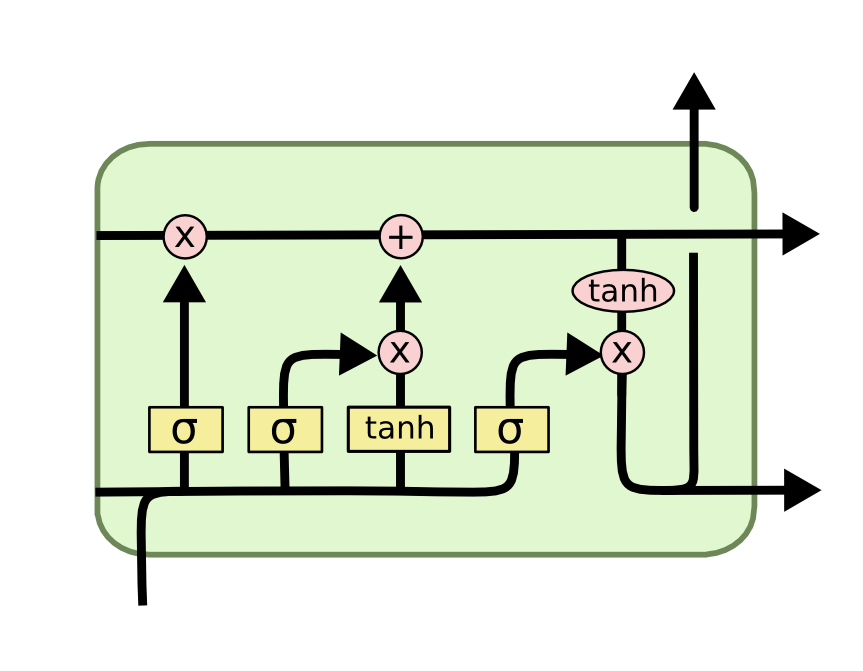
\includegraphics[width=\columnwidth, keepaspectratio]{LSTMChain}
	\caption{LSTM as Conscious \& Subconscious of AI}
	\label{Fig:fig4}
\end{figure}

The LSTM architecture consists of several specialized gates that control the flow of information as show in figure \ref{Fig:fig4}. These gates include the input gate, forget gate, output gate, and cell update gate. Each gate is composed of a sigmoid activation function, which determines the amount of information to be passed through. If we observe the working of the LSTM-RNN, we can understand that when a sequential data pattern repeats frequently, the LSTM stores it in a separate cell known as the memory cell$ (c_{t-1}) $ present within its architecture, just like the human subconscious mind forms habits by performing consciously repeating actions and patterns of life.